\section{完成情况及性能参数}
\label{sec:results}

\subsection{整体介绍}
作品已搭建由OS-ZYNQ7100开发板、OV9281相机、HDMI显示器和串口屏组成的实验系统，如图\ref{fig:system-photo}所示。相机安装在可调支架上，对准扬声器膜片；开发板完成图像处理与控制，HDMI显示器呈现视频结果，串口屏提供参数设置和启停操作。实验仪器用于产生和观察激励信号。系统采用现成板卡和外围设备，设计重点为图像算法的FPGA实现及采集、处理、显示和控制的联调。

\reportfig{system-overview.png}{0.82}{系统实验布置实物照片，包含被测扬声器、相机、开发板、串口屏、显示器及实验仪器。}{fig:system-photo}

\subsection{工程成果}
\subsubsection{机械成果}
相机采用现成支架固定，可调整高度与观察方向，使扬声器膜片位于成像范围内。开发板和显示终端采用桌面布置，便于接线、调试与操作。相机支架与被测物保持相对稳定，以减少拍摄装置晃动引入的图像位移。

\subsubsection{电路成果}
硬件集成完成相机输入、HDMI输出、串口交互和供电连接，复用开发板上的处理器、DDR及QSPI存储。板内逻辑由HLS计算IP和RTL视频通路组成，PS驱动程序负责设备配置与任务调度。外围接口与片上模块共同构成从图像采集到显示输出的处理链路。

\subsubsection{软件成果}
串口屏主界面如图\ref{fig:hmi-interface}所示。左侧选择原画、放大画面及详细参数视图，右侧调节相位增益和相机曝光，下方显示设备状态并提供启动入口。数值框承载用户设定，状态栏呈现设备反馈。增益生效以寄存器读回和新参数帧处理完成为判据，曝光生效以启动时的相机配置读回为判据，具体测试结果见第\ref{sec:interaction}节。

\reportfig{hmi-interface.png}{0.85}{串口屏主操作界面，包含视图选择、相位增益、相机曝光和启停控制。}{fig:hmi-interface}

\subsection{特性成果}
\subsubsection{测试环境与版本说明}
本文代码版本为V19（\texttt{v19boot}），整理后的工程固定于提交\texttt{a9ab041021c2}；2021.2与2025.2表示AMD工具版本。实验以扬声器为被测对象，检测固定ROI内的运动，并展示整帧相位运动放大结果。本节按测试版本列出板级运行结果、启动结果及Vivado~2025.2构建结果，见表\ref{tab:evidence-versions}。各项测试的原始数据和日志可通过仓库证据索引查阅\cite{repo}。

\begin{table}[htbp]
\centering\small
\caption{测试版本、条件与结果对应关系}\label{tab:evidence-versions}
\begin{tabularx}{\linewidth}{@{}p{2.7cm}p{3.2cm}X@{}}
\toprule
测试版本或材料 & 主要条件 & 已完成内容 \\
\midrule
扬声器双频实验 & 5\,Hz与10\,Hz激励，256个连续位移样本 & 对照设定频率检查位移谱峰 \\
v18hmi板级实验 & 串口交互、32分钟固定参数运行 & 命令响应及处理/显示速率测量 \\
v19补充验收 & 2021.2产物，11月3日三次断电上电及现场交互 & 冷启动、程序读回、KEY0、触屏与STOP确认 \\
黄金参考/C模型 & 两种尺寸，四组相位增益，同输入与帧映射 & 逐像素误差比较；输出来自HLS C仿真 \\
2025.2基线构建 & 提交\texttt{a9ab041021c2}及配套导出IP & 主机回归、RTL比对、硬件实现、固件编译及启动包静态检查 \\
实验场景图片 & 整机布置、原画与放大输出、串口屏界面 & 展示实物组成、显示模式和操作入口 \\
\bottomrule
\end{tabularx}
\end{table}

作者已确认整机上板可用。本节按实际来源区分证据：双频实验提供频谱记录，v18hmi提供固定配置连续运行和交互数据，11月3日的v19/2021.2记录提供补充验收结果，Vivado~2025.2基线提供资源与内部时序报告。不同版本分别保留，不将v19实测转记为2025.2构建产物的测量结果。

\subsubsection{运动放大效果}
图\ref{fig:display-comparison}展示同一扬声器场景的原画与放大输出。原画模式呈现相机采集的灰度图像，放大模式呈现相位处理后的图像；两种模式均叠加红色ROI框，标示原始帧中用于位移估计的固定区域。

\begin{figure}[htbp]
\centering
\begin{minipage}[t]{0.485\linewidth}
\centering
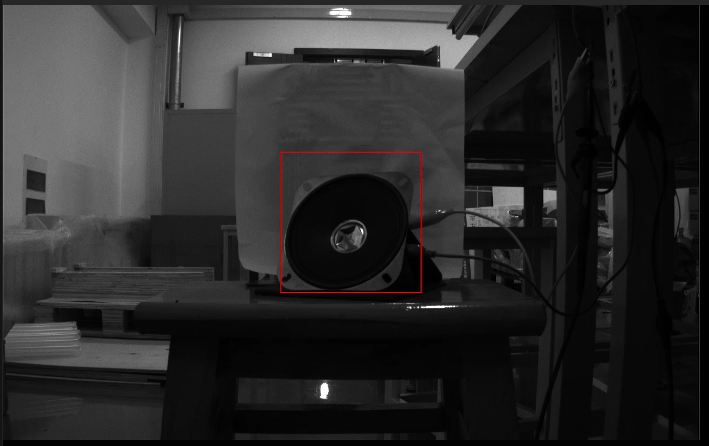
\includegraphics[width=\linewidth]{figures/display-original.png}
\par\small （a）原画面
\end{minipage}\hfill
\begin{minipage}[t]{0.485\linewidth}
\centering
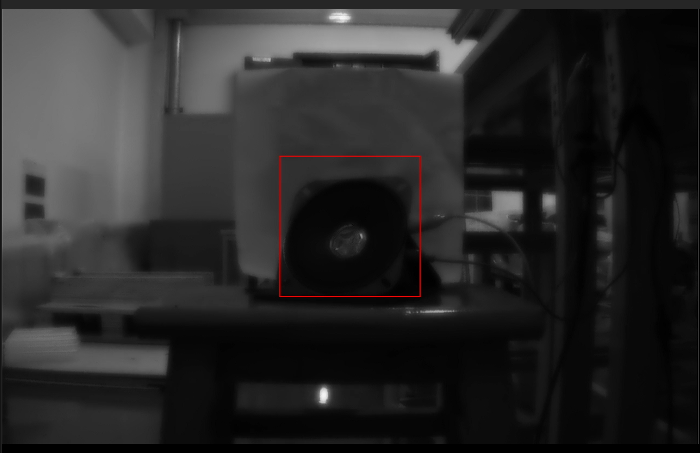
\includegraphics[width=\linewidth]{figures/display-amplified.png}
\par\small （b）放大输出画面
\end{minipage}
\caption{扬声器场景的原画与相位运动放大输出。两幅静态截图展示显示模式，红框标示固定ROI。}
\label{fig:display-comparison}
\end{figure}

系统将可视化与测量分开处理：运动放大支路生成显示图像，ROI支路直接从原始帧估计位移。本文位移及谱幅采用像素单位，$\alpha$表示相位调制强度；本节静态图比较不用于确定物理位移放大倍率。

\subsubsection{黄金参考与C模型数值比较}
补充数值比较使用同一输入、参数与帧映射，将独立黄金参考与HLS C模型输出逐像素对应。测试覆盖$64\times64$的128帧序列和$1280\times800$的8帧序列，均取$\alpha=0,12,30,50$。两组已归档样例的最大绝对误差均不超过1个RAW10码值。全尺寸结果见表\ref{tab:golden-comparison}，MAE与RMSE分别为全部像素的平均绝对误差和均方根误差。

\begin{table}[htbp]
\centering\small
\caption{全尺寸8帧黄金参考与HLS C模型输出比较}\label{tab:golden-comparison}
\begin{tabular}{@{}rrrr@{}}
\toprule
$\alpha$ & MAE & RMSE & 最大绝对误差 \\
\midrule
0 & 0 & 0 & 0 \\
12 & $1.2207\times10^{-7}$ & $3.4939\times10^{-4}$ & 1 \\
30 & $6.0168\times10^{-4}$ & $2.4529\times10^{-2}$ & 1 \\
50 & $8.0566\times10^{-6}$ & $2.8384\times10^{-3}$ & 1 \\
\bottomrule
\end{tabular}
\par\smallskip
\begin{minipage}{\linewidth}\small
注：误差单位为RAW10码值，像素范围0至1023。输出来源为主机HLS C仿真，非物理FPGA像素采集。
\end{minipage}
\end{table}

输入、参考、输出、逐帧误差与来源哈希由\path{board/results/v19_acceptance_20261103/}下的\path{golden_validation/}及\path{golden_validation_full/}索引，原始数组保存在完整验收附件。该比较验证所列样例的数值对应关系，不用于推导端到端延迟、实际位移放大倍率或板端逐像素误差。

\subsubsection{振动频率检测结果}
双频实验以5\,Hz和10\,Hz信号驱动扬声器，比较设定频率与图像位移谱峰的位置。固定ROI为$256\times256$，左上角坐标为$(512,272)$；时间谱由256个连续有效位移样本计算。

频谱读取程序重复读取结果缓冲区，并核对结果序号，仅接收两次读取一致的快照。9个候选快照中有3个满足该条件。图\ref{fig:spectrum-result}采用\texttt{spectrum\_00}：实测采样率为60.37956\,Hz，频点间隔约0.23586\,Hz，时间窗约4.24\,s；5\,Hz和10\,Hz附近的局部峰分别位于第21和42个频点，对应4.95301\,Hz和9.90602\,Hz，与输入频率对应。

\reportfig{fig3-5-spectrum.pdf}{1.0}{扬声器双频实板实验的ROI位移谱。纵轴为图像位移谱幅（px）；绘图保留原始频点，直流和奈奎斯特端点按单边谱定义修正，未作平滑或最大值归一化。}{fig:spectrum-result}

表\ref{tab:frequency-peaks}列出3个一致快照的插值峰值。六个峰值相对设定频率的绝对偏差为0.00231至0.02418\,Hz，说明该工况下能够分辨5\,Hz与10\,Hz输入。各快照取自同一连续采集过程，窗口可能重叠，表中偏差按快照列示，不作为独立重复测量的精度统计。图中约15、20、25、30\,Hz附近的附加分量保留在完整频谱中。

\begin{table}[htbp]
\centering\small
\caption{一致性通过快照中的频率峰值}\label{tab:frequency-peaks}
\begin{tabular}{@{}lrrr@{}}
\toprule
快照 & 目标频率/Hz & 插值峰值/Hz & 绝对偏差/Hz \\
\midrule
\texttt{spectrum\_00} & 5 & 5.01217 & 0.01217 \\
\texttt{spectrum\_00} & 10 & 10.00324 & 0.00324 \\
\texttt{spectrum\_05} & 5 & 5.02418 & 0.02418 \\
\texttt{spectrum\_05} & 10 & 10.00623 & 0.00623 \\
\texttt{spectrum\_06} & 5 & 5.00818 & 0.00818 \\
\texttt{spectrum\_06} & 10 & 9.99769 & 0.00231 \\
\bottomrule
\end{tabular}
\end{table}

\subsubsection{交互功能与边界测试}
\label{sec:interaction}
v18hmi交互实验通过真实UART链路测试\texttt{VIEW}、\texttt{ALPHA}、\texttt{EXPOSURE}、\texttt{START}和\texttt{STOP}五类命令。自动测试持续602631\,ms，共完成30轮交互；现场观察另记录了部分按键与屏幕操作。表\ref{tab:interaction-results}分别列出命令行为和验证方式。

\begin{table}[htbp]
\centering\small
\caption{v18hmi交互测试结果}\label{tab:interaction-results}
\begin{tabularx}{\linewidth}{@{}p{2.2cm}X p{3.1cm}@{}}
\toprule
动作 & 已记录行为 & 验证方式 \\
\midrule
VIEW切换 & 三视图与反馈状态对应；停止时切换不隐含启动 & 串口记录及部分现场确认 \\
ALPHA设置 & 范围与非法输入受控；新帧完成并读回匹配后确认 & 串口测试、增益操作反馈 \\
EXPOSURE设置 & 空闲时排队，下次启动应用；运行中返回BUSY & 串口测试及现场流程确认 \\
START / STOP & 就绪后报运行，排空后报停止；取消待执行重启 & 串口链路与状态读回 \\
按键与屏幕 & 视图同步，键盘编辑期间保护未提交内容 & 对应操作的现场观察记录 \\
\bottomrule
\end{tabularx}
\end{table}

曝光设置采用排队应用机制：空闲时保存新设定，启动采集前写入相机并核对读回值；运行中收到曝光修改请求时返回\texttt{BUSY}。停止后显示器可保持末帧，参数是否生效由设备反馈确认。

11月3日的v19补充记录保存了触屏切换至放大加频谱视图、KEY0两次切换及STOP操作。KEY0按下、受理和完成计数均为2；作者确认HDMI视图切换后恢复，STOP后屏幕显示停止且画面保持。三次真实断电上电均进入默认STOPPED状态，QSPI启动状态和运行程序读回相符。该补充记录按BOOT、位流、ELF和板内应用代码SHA256关联，入口为\path{board/results/v19_acceptance_20261103/README.md}。

\subsubsection{连续运行与处理速率}
v18hmi在VIEW~2、$\alpha=50$、曝光参数320的固定条件下连续运行32分钟。193个遥测采样点形成192个相邻区间，间隔约10\,s；处理帧计数增加115929，显示完成计数增加57600。按计数增量除以1920\,s计算，平均处理速率为60.37969\,frame/s，显示速率为30.00000\,frame/s。图\ref{fig:runtime-result}给出各区间结果，全程采集、算法及序列不连续等错误计数均为0。

\reportfig{fig3-6-runtime.pdf}{1.0}{v18hmi连续32分钟运行的区间处理与显示速率。阶梯线由计数差和时间差计算，虚线为时间加权平均；两面板纵轴跨度均为2\,frame/s。}{fig:runtime-result}

该结果表明，在上述输入和参数下，系统能够持续完成图像处理与30\,frame/s显示。曲线中的区间速率用于描述约10\,s尺度上的吞吐变化，上述计数不用于换算单帧端到端延迟。

v19补充记录的首尾计数跨度为2418.1\,s，处理计数增加146004，平均约60.3796\,frame/s；显示完成计数速率为30.0\,Hz，频谱发布约4.9857次/秒。该跨度包含234.1\,s的未观测间隙，期间存在调参和两次JTAG采集中断；累计有效观测为2184\,s。因此这些数据仅作为该版本板内计数端点速率，不替代v18固定配置32分钟连续运行结果，也不记为连续60分钟验收通过。

\subsubsection{FPGA资源利用率与实现约束分析}
\paragraph{实现后资源总量}
资源统计针对目标器件\texttt{xc7z100ffg900-2}上的完整设计\texttt{capture\_wrapper}，以Vivado~2025.2布局布线后的Physopt postRoute报告为准。图\ref{fig:utilization-result}直观展示各类资源的利用率，表\ref{tab:resource-total}给出精确数量。综合与实现报告为分析器件内映射和时序的依据\cite{ug901,ug904}。

\reportfig{utilization.png}{0.78}{FPGA资源利用率界面概览，百分比为取整显示；2025.2基线的精确数量与统计口径见表\ref{tab:resource-total}。}{fig:utilization-result}

\begin{table}[htbp]
\centering\small
\caption{2025.2完整设计的实现后资源占用}\label{tab:resource-total}
\begin{tabular}{@{}lrrr@{}}
\toprule
资源 & 已用数量 & 可用总量 & 利用率/\% \\
\midrule
LUT & 138026 & 277400 & 49.76 \\
LUT as Memory & 13029 & 108200 & 12.04 \\
FF & 206397 & 554800 & 37.20 \\
BRAM Tile & 744.5 & 755 & 98.61 \\
DSP & 826 & 2020 & 40.89 \\
Bonded IOB & 25 & 362 & 6.91 \\
BUFGCTRL & 4 & 32 & 12.50 \\
MMCME2\_ADV & 1 & 8 & 12.50 \\
\bottomrule
\end{tabular}
\par\smallskip
\begin{minipage}{\linewidth}\small
注：LUT as Memory包含在LUT总量内，不能重复相加；其中1424个用于分布式RAM、11605个用于移位寄存器。BRAM按36\,Kb Tile等效量统计。
\end{minipage}
\end{table}

\paragraph{片上存储与模块分摊}
BRAM使用744.5/755个Tile，容量余量为10.5个Tile，约1.39\%。其中708个RAMB36与73个RAMB18按$708+73/2$换算得到744.5个Tile。片上存储是利用率最高的主要资源，扩展缓存或增加ROI时应优先评估其容量和布局位置；DDR带宽则需依据访问量和运行测量单独分析。

表\ref{tab:resource-modules}按模块列出资源开销。运动放大模块使用391个BRAM Tile和557个DSP，ROI模块使用266个BRAM Tile和61个DSP，两者合计使用657个BRAM Tile，占已用BRAM的88.25\%，是存储优化的重点。表中四个模块合计使用673.5个BRAM Tile，占全设计BRAM用量的90.46\%，并包含全部826个DSP。完整设计还集成了离线时间滤波模块，其资源单独列入\texttt{f}实例。

\begin{table}[htbp]
\centering\small
\caption{主要模块的实现后资源分摊}\label{tab:resource-modules}
\begin{tabular}{@{}lrrrr@{}}
\toprule
模块及功能 & LUT & FF & BRAM Tile & DSP \\
\midrule
\texttt{motion}：运动放大 & 77542 & 117613 & 391 & 557 \\
\texttt{roi}：位移估计 & 8582 & 12084 & 266 & 61 \\
\texttt{spec\_fft}：时间频谱 & 4820 & 6853 & 6.5 & 12 \\
\texttt{f}：离线时间滤波 & 21461 & 31771 & 10 & 196 \\
\bottomrule
\end{tabular}
\par\smallskip
\begin{minipage}{\linewidth}\small
注：取同层实例统计，已包含各自子模块；不与下级资源再次累计。跨层次LUT合并可能影响子级加总，整体占用以顶层报告为准。
\end{minipage}
\end{table}

\paragraph{布局时序与扩展代价}
LUT、FF和DSP利用率分别为49.76\%、37.20\%和40.89\%，Slice占用为58571/69350，即84.46\%。功能扩展需要同时考虑资源组合、布局位置和布线需求。现有约束覆盖的内部时序中，WNS为$+0.177$\,ns、WHS为$+0.010$\,ns，TNS与THS均为0，建立与保持时序检查通过。MIPI~HS和HDMI的板外接口裕量不在该内部时序结果的覆盖范围内。

上述结果表明，完整基线设计已在目标器件上完成布局布线，BRAM是后续扩展的主要容量约束。优化方向为缩短缓存生存期、复用片上工作区，并结合数值误差评估存储位宽；评价时同时记录资源变化、输出误差、处理速率和时序余量。

\subsubsection{仿真回归与启动验证}
工程采用主机回归、软件/RTL比对、硬件实现和启动检查组成的验证流程，结果见表\ref{tab:validation-results}。主机回归检查协议与调度逻辑，软件/RTL比对检查频谱显示输出，综合实现检查资源映射和内部时序，启动包检查确认硬件平台与固件的配套关系。

\begin{table}[htbp]
\centering\small
\caption{验证层次及已完成范围}\label{tab:validation-results}
\begin{tabularx}{\linewidth}{@{}p{3.1cm}X p{4.1cm}@{}}
\toprule
验证项目 & 测试结果 & 检查对象 \\
\midrule
主机回归 & 8项测试通过 & 协议解析与调度逻辑 \\
频谱UI软件/RTL & Vivado~2025.2比对通过 & 软件参考与RTL显示结果的一致性 \\
2025.2基线实现 & 71个IP及顶层综合、布局布线和产物导出通过 & 完整基线设计的资源和内部时序 \\
固件与启动包 & 应用、FSBL构建及BOOT三分区静态检查通过 & 平台配置、分区组成及应用载荷 \\
v19补充验收 & 三次冷启动、KEY0两次操作及STOP检查通过 & 程序读回、计数记录与现场确认 \\
黄金参考/C模型 & 两种尺寸、四组增益；最大绝对误差不超过1 & 已归档HLS C输出，非板端像素输出 \\
HLS重生成阶段 & 五个模块C仿真、生产综合、导出及声明接口核对完成 & 原版源码；RTL与系统实现范围见下文 \\
\bottomrule
\end{tabularx}
\end{table}

11月3日19:48的HLS结果快照以原版提交\texttt{a9ab041021c2}为输入，使用Vitis HLS~2025.2、器件\texttt{xc7z100ffg900-2}和6.666667\,ns目标周期。五个模块已完成C仿真、生产配置综合与IP导出，声明接口核对一致；接口一致不等同于内部功能或实现时序等价。

RTL联合仿真中，复制模块以10组独立仿真、21次调用覆盖12个案例及11组相邻关系；频谱模块完成311个事务；时间滤波模块完成有界分组11次调用，AXI深度为15360，不外推至生产地址范围。ROI模块通过两个参数拒绝分支，正常路径尚未完成；运动放大模块已完成全尺寸C测试，完整帧RTL运行因资源限制中止。新候选IP的系统集成实现仍在进行，未纳入本文已通过的整机资源和时序结论。

各项测试保留输入、输出和结果记录，并将源码、硬件平台、位流、固件及启动包按版本关联归档。上述HLS阶段结论固定于所注明快照，完整验证及后续实现结果在完成后单独整理。

\subsubsection{资源优化设计与工程改进}
\paragraph{计算与存储的设计取舍}
表\ref{tab:design-tradeoffs}列出计算与存储的组织方法及其代价。设计以局部数据复用、紧凑状态布局和独立任务调度支撑连续视频处理，同时保留浮点算法的数值形式。

\begin{table}[htbp]
\centering\small
\caption{面向FPGA的计算与存储设计取舍}\label{tab:design-tradeoffs}
\begin{tabularx}{\linewidth}{@{}p{2.5cm}X X@{}}
\toprule
设计选择 & 具体组织与作用 & 资源及调度代价 \\
\midrule
行缓存与流水连接 & 空间邻域复用行缓存，算子间以FIFO传递数据 & 占用片上存储，FIFO深度需匹配各级启动和处理节奏 \\
相位状态紧凑存储 & 四组96位状态占三个128位AXI字，减少填充位 & 增加打包与解包逻辑，内部计算流保持原有接口形式 \\
共享原始帧与双支路 & 放大和ROI任务读取同一采集帧，分别维护完成状态 & 两路均释放输入后才能复用原始帧，需协调DDR访问与任务完成事件 \\
浮点运算与专用资源 & 相位、滤波及位移处理采用浮点计算并映射至PL & 浮点算子占用DSP与逻辑，位宽调整需同步评估数值误差 \\
\bottomrule
\end{tabularx}
\end{table}

在线模式的源码为每个像素保存参考相位与两个IIR状态，共$3\times32=96$位；四个像素共384位，打包为三个128位AXI字。相较每像素占用一个128位字的布局，该组织减少了状态填充位，并保持原有内部计算流接口。状态布局的作用是提高存储有效载荷比例，完整设计的资源占用见表\ref{tab:resource-total}。

\paragraph{已验证的工程修正}
串口接收、数值回包及重启状态管理中的问题和修正见表\ref{tab:engineering-revisions}。这些改进针对命令及时接收、数据访问约束及状态初始化，使控制流程与设备实际运行状态保持一致。

\begin{table}[htbp]
\centering\small
\caption{已记录的工程修正及验证范围}\label{tab:engineering-revisions}
\begin{tabularx}{\linewidth}{@{}p{3cm}X X@{}}
\toprule
原问题 & 实施处理 & 回归或实现结果 \\
\midrule
UART短包停留FIFO & RX触发阈值设为1，中断内排空FIFO & 对应主机及真实串口命令测试通过 \\
非对齐数值回包出错 & ARM构建保留禁止非对齐访问选项 & 对应版本重新测试通过 \\
空闲超时触发接收中断 & 禁用RX空闲超时，保留数据接收中断 & 接收处理由有效数据触发，减少空闲状态下的中断处理 \\
重启后遥测继承旧值 & 清零保留区并初始化中断、计时器状态 & v19交接及冷启动记录确认对应修正 \\
\bottomrule
\end{tabularx}
\end{table}

本节以设计结构和回归结果说明工程改进，以板级计数和实现报告分别给出吞吐及资源数据。后续量化优化收益时，应固定器件、工具、输入、参数和约束，在同一计时方法下比较输出误差、处理速率、BRAM/DSP占用及时序余量。

\subsubsection{工程复现与材料组织}
\label{sec:reproduction}
项目源码仓库为\url{https://github.com/cuijiaxin269-svg/FPGA_Visual_amplifier}，包含RTL、HLS与PS源码、构建脚本和验证记录。配套发布附件及使用方法见仓库README。完整演示视频与文件哈希见\path{media/video_manifest.json}；作者AI协作总结见\path{report/ai_logs/author_collaboration_summary_20261103.md}。11月3日配套资料的发布说明见\path{report/design_report/PUBLICATION_NOTE.md}，资料通过\texttt{materials-20261103}发布入口获取。

报告对应的代码基线为V19（\texttt{v19boot}）整理版，固定于提交\texttt{a9ab041021c2}；资源与时序来自该基线的Vivado~2025.2重新构建。完整提交号及文件哈希保存在配套清单中。已核对该提交的825项硬件输入、58项主机测试输入、6项频谱RTL验证输入和43项固件输入，均与构建记录的SHA256一致。重建原版工程时在独立目录检出该提交，并使用对应的位流、XSA、初始化文件和固件。该提交用于固定工程源码，11月3日新增的验收、黄金参考、屏端与硬件、视频及AI总结随当前资料版本提供；两者分别记录版本和哈希。

构建环境为Windows、AMD~2025.2工具、Python~3及包含标准头文件与库的C++工具链。硬件重建采用归档的导出IP；软件、仿真与硬件输出分别写入独立目录，保留各阶段结果。表\ref{tab:reproduction}列出执行顺序、入口和通过判据，命令参数及路径配置见仓库README和构建说明\cite{repo}。

\begin{table}[htbp]
\centering\small
\caption{工程复现顺序、入口与判据}\label{tab:reproduction}
\begin{tabularx}{\linewidth}{@{}p{2.0cm}p{6.5cm}X@{}}
\toprule
步骤 & 仓库内入口 & 通过判据 \\
\midrule
来源与文件核对 & \path{build/scripts/verify_package.py}\newline\path{report/evidence_index.md} & 文件清单、IP引用与目标版本一致 \\
主机及RTL验证 & \path{sim/scripts/run_host_tests.py}\newline\path{sim/scripts/run_spectrum_rtl.py} & 对应结果记录通过，保留输入和比较输出 \\
固件及硬件构建 & \path{build/scripts/build_firmware.py}\newline\path{build/scripts/build_hardware.ps1} & 检查结果记录、实现资源、约束内时序及导出产物 \\
启动包配套 & \path{build/scripts/build_boot.py} & XSA、位流、应用与FSBL成套，镜像检查和哈希一致 \\
实板功能验证 & \path{board/}及\path{report/evidence_index.md}中的对应版本记录 & 逐项确认采集、三视图、交互、停止排空及冷启动；保存实际日志 \\
\bottomrule
\end{tabularx}
\end{table}

重新构建或更换版本后的板级复测，应记录位流和ELF哈希、输入激励、ROI、曝光、相位增益、运行时长及判据。处理速率按处理帧计数增量计算，显示速率按显示完成计数计算；频谱检查应保存原始位移样本、窗口参数及数值结果。复测采集时，应按输入帧序号保存原画与处理输出，便于进一步分析位移与运动增强效果。

各阶段结果记录包含执行状态、输入文件哈希、输出位置和错误信息；通过版本清单将测试输入、构建产物与运行记录关联，便于复查设计结果和定位复现过程中出现的问题。
